\chapter{Jezyki i~technologie webowe}
\PartialToc
%\startcontents[chapters]
%\printcontents[chapters]{}{1}{\section*{\contentsname}}

%%% PYTANIE 148
\answer
{Ile zasobów z dyrektywami CSS może być skojarzonych z pojedynczym dokumentem XHTML 1.0 Strict?}
{Zero}
{F}
{Nie ma ograniczenia dołączanych plików styli.}
{Nie ma czego wyjaśniać.}


%%% PYTANIE 149
\section{Zaznacz prawdziwe stwierdzenia dotyczące poniższego kodu CSS 2.1.}
\begin{lstlisting}[language=html]
.nav > div {
	color: white;
	background: #119500;
	float: right;
	width: 120px;
	padding: 1px;
	font-size: small;
	border: solid red 1px;
}
\end{lstlisting}

\noindent
{\textbf{Przykładowa odpowiedź:}}
Kolor tła ustalony jest jako wartości składowych RGB, odpowiednio (dziesiętnie) 11, 95, 0.
\textbf{FAŁSZ}

\vspace{0.4cm}
\noindent
\textbf{Odpowiedź:}
Brak jednoznacznej odpowiedzi.

\vspace{0.4cm}
\noindent
\textbf{Wyjaśnienie:}

Powyższa definicja styli dotyczy elementu div, będącego bezpośrednim potomkiem elementu z klasą nav (znaczenie selektora \textbf{>}).
Na przykład:
\begin{lstlisting}[language=html]
<div class="nav">
	<div id="stylowanyDiv"></div>
</div>
\end{lstlisting}

Tu stylowanie nie będzie miało miejsca:

\begin{lstlisting}[language=html]
<div class="nav">
	<span>
		<div id="nieBedeStylowany"></div>
	</span>
</div>
\end{lstlisting}


\begin{itemize}
\item
\textbf{color} - kolor tekstu wewnątrz elementu; w tym przypadku tekst będzie BIAŁY.
\item
\textbf{background} - tło elementu; tutaj ustawiony kolor tła jako wartość HEX koloru. Chcąć ustawiać kolor jako dziesiętne wartości RGB używamy formy rgb(R, G, B)
\item
\textbf{float} - w najprostszej formie określa czy i jak element będzie 'opływany' przez tekst; tutaj, div będzie znajdował się po prawej stronie, a tekst z lewej.
\item
\textbf{width} - szerokość elementu blokowego; tutaj, 120 px
\item
\textbf{padding} - jest odstępem między zawartością elementu a jego wewnętrzną krawędzią; tutaj, 1px dla wartości górnej, prawej, dolnej i lewej jednakowo.
\item
\textbf{font-size} - rozmiar tekstu; tutaj, mniejsza niż domyślna. Dokładny rozmiar jest zależny od przeglądarki.
\item
\textbf{border} - obramowanie elementu; solid - linia ciągła, red - czerwony kolor obranowania, 1px - grubość obramowania;
\end{itemize}
\begin{center}
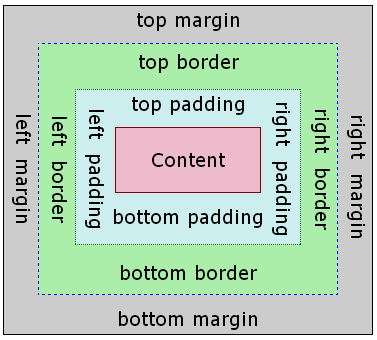
\includegraphics[width=6cm]{09/boxmodel}
\captionof{figure}{Model pudełkowy elementów strony}
\end{center}

\textbf{!UWAGA!: }120px jest poprawne; 120 px już nie!


%%% PYTANIE 150
\section{Wskaż prawdziwe stwierdzenia odnośnie poniższego fragmentu kodu PHP.}
\begin{lstlisting}[language=php]
$fp = fopen("plik_do_blokowania", "r+");
if(flock($fp, LOCK_EX)) {
	processing();
	flock($fp, LOCK_UN);
} else {
	problem();
}
fclose($fp);
\end{lstlisting}

\noindent
{\textbf{Przykładowa odpowiedź:}}
Funkcja \textit{processing()} jest wywoływana w sekcji krytycznej.
\textbf{PRAWDA}

\vspace{0.4cm}
\noindent
\textbf{Odpowiedź:}
Brak jednoznacznej odpowiedzi.

\vspace{0.4cm}
\noindent
\textbf{Wyjaśnienie:}

\begin{enumerate}
\item 
Funkcja \textit{fopen} przyjmuje jako pierwszy argument ścieżkę do pliku, który ma zostać otwarty, a jako drugi - tryb otwarcia, jak niżej:
\begin{itemize}
\item
\textbf{r} - otwiera plik do odczytu
\item
\textbf{r+} - otwiera plik do odczytu i zapisu
\item
\textbf{w} - kasuje zawartość pliku i otwiera go do zapisu
\item
\textbf{w+} - kasuje zawartość pliku i otwiera go do zapisu i odczytu
\item
\textbf{a} - otwiera plik do dopisywania
\item
\textbf{a+} - otwiera plik do dopisywania i odczytu
\end{itemize}
Zwraca wartość liczbową identyfikującą otwarty plik.
\item
Funkcja \textit{fclose} służy do zamknięcia pliku otwartego wcześniej przez fopen. Jako argument przyjmuje liczbowy identyfikator pliku, który ma zostać zamknięty.
\item
Funkcja \textit{flock} służy do zarządzania blokowaniem dostępu do pliku jako zabezpieczenie podczas współdzielenia pliku. Zapobiega to równoczesnej modyfikacji pliku przez kilka osób/wątków.
\begin{itemize}
\item
\textbf{LOCK\_SH} - dostęp do odczytu; inne wątki mogą czytać plik, ale nie mogą zablokować go do zapisu. Zapobiega to odczytowi niepełnych danych przez inne wątki i wprowadzeniu zmian w pliku czytanym przez inne wątki.
\item
\textbf{LOCK\_EX} - dostęp do zapisu; wątek blokując plik w ten sposób ma go 'na wyłączność'. Inne wątki nie mogą go odczytać, a tym bardziej zapisać. Zapobiega wprowadzaniu zmian przez kilka wątków jednocześnie oraz odczytania niepełnych (przed edycją) danych.
\item
\textbf{LOCK\_UN} - zwolnienie blokady 
\item
\textbf{LOCK\_NB} - Gdy ustawiona, proces który natknął się na blokadę nie będzie czekał na swoją kolej. Używa się tej opcji w połączeniu, z którąś opcją blokady np. \textit{flock(\$fp, LOCK\_EX | LOCK\_NB)}. Użyta w naszym przypadku pozwoliła by na przejście bo bloku \textit{else} gdy plik jest już zablokowany, zamiast czekać na zwolnienie.\textbf{LOCK\_UN}
\end{itemize}
\textit{flock} zwraca true w przypadku sukcesu i false w przeciwnym razie.
Gdy \textit{flock} nie może uzyskać do zasobu, oczekuje na zwolnienie blokady przez inny wątek!

Funkcja \textit{flock} może przyjmować także opcjonalnie trzeci parametr. Jego wartość jest ustawiana jako 1, gdy proces zostanie zablokowany (nie uzyska dostępu do pliku). Głównie służy do sprawdzenia czy coś złego się nie wydarzyło - gdy funkcja zwraca \textbf{false}, a trzeci parametr ma wartość 0, oznacza to że wystąpił jakiś błąd, ponieważ \textit{flock} nie mógł uzyskać blokady, a jednak proces nie został wstrzymany przez już istniejącą blokadę na pliku.
\end{enumerate}


\textbf{Analiza kodu:}
\begin{enumerate}
\item
Otwieramy plik "plik\_do\_blokowania" w celu odczytu i zapisu. Identyfikator przypisujemy do zmiennej \$fp.
\item
Następnie próbujemy uzyskać dostęp do pliku w trybie exclusive.
Jeżeli plik nie został wcześniej zablokowany ani do odczytu, ani zapisu przez inny wątek - funkcja \textit{flock} zwraca \textbf{true} i blokuje plik.
\item
Wówczas wchodzimy w sekcję krytyczną gdzie aktywowana jest funkcja \textit{processing()}.
\item
Po jej wykonaniu blokada pliku jest zwalniana poprzez \textit{flock(\$fp, LOCK\_UN)}.
\item
Jeżeli plik jest odczytywany lub zapisywany przez inny wątek (został wcześniej zablokowany) funkcja \textit{flock} zwraca \textbf{false}.
Wówczas \textit{flock} oczekuje na zwolnienie blokady przez inny wątek; czeka na swoją kolej.
\item
Po wykonaniu powyższych czynności plik zostaje zamknięty.
\end{enumerate}

\textbf{!Uwaga!: }Tak naprawdę, w tym przykładzie nie wejdziemy do bloku 'else'!

%%%% Pytanie 151
\section{Zawartość poniższego formularza przesłano do skryptu PHP. Zaznacz prawdziwe stwierdzenia.}
\begin{lstlisting}[language=html]
<form action="skrypt.php" method="post" enctype="multipart/form-data">
	<p>
		<input type="file" name="plik"/>
		<input type="text" name="comment" />
		<input type="submit" value="wyslij" />
	</p>
</form>
\end{lstlisting}

\noindent
{\textbf{Przykładowa odpowiedź:}}
W zmiennej \textit{\$\_POST['comment']} będzie dostępna zawartość pola tekstowego.
\textbf{PRAWDA}

\vspace{0.4cm}
\noindent
\textbf{Odpowiedź:}
Brak jednoznacznej odpowiedzi.

\vspace{0.4cm}
\noindent
\textbf{Wyjaśnienie:}
Formularz php składający się z trzech elementów:
\begin{enumerate}
\item
Kontrolka do uploadu pliku. Klikając klawisz pojawi się okno eksploratora i można wybrać plik z dysku. Zmienna z nim związana nazwana została 'plik'.
\item
Pole tekstowe, umożliwiające wpisanie tekstu przez użytkownika. Pierwotnie pole tekstowe jest puste. Zmienna z nim związana nazwana została 'comment'.
\item
Klawisz zatwierdzający formularz. Po jego wciśnięciu dane z formularza zostają wysłane do skryptu 'skrypt.php' metodą POST.
\end{enumerate}

Parametr \textbf{enctype} określa w jaki sposób dane z formularza zostaną przekształcone. Może być użyty TYLKO w połączeniu z \textbf{method="POST"}.
	Możliwe wartości:
\begin{itemize}
\item
\textbf{application/x-www-form-urlencoded} - DOMYŚLNE; Wszystkie dane są przekształcane. Spacje zmieniane na +, znaki specjalne zmieniane na wartości ASCII HEX.
\item
\textbf{multipart/form-data} - żadne znaki nie są przekształcane; wymagany w przypadku użycia w formularzu kontrolki typu \textbf{'file'}
\item
\textbf{text/plain}- spacje są przekształcane na znak +, znaki specjalne nie są przekształcane
\end{itemize}

Po stronie skryptu php dostępne są wartości z tablicy asocjacyjnej \textit{\$\_POST} (pola z formularza z metodą \textbf{POST}; przy użyciu metody \textbf{GET} wartości dostępne są spod \textit{\$\_GET}) oraz \textit{\$\_FILES} (dane z kontrolki typu \textbf{file}).

\begin{itemize}
\item
\$\_POST: Array ([comment] => <tresc\_komentarza\_wpisana\_w\_polu>)
\item
\$\_FILES: Array ([plik] => Array ([name] => <nazwa\_pliku> [type] => image/png [tmp\_name] => <sciezka\_do\_pliku\_w\_tempie> [error] => 0 [size] => 38676))
\end{itemize}
Do elementów dostać się można na przykład: \textit{\$\_POST['comment']}, \textit{\$\_FILES['plik']['name']}.

Elementy formularza zgrupowane są wewnątrz znacznika akapitu (<p>).
